\chapter{Конструкторский раздел}
\section{Проектирование БД}
\subsection{Описание сущностей проектируемой базы данных}
База данных состоит из 6 табилиц:
\begin{enumerate}[label=\arabic*)]
	\item Таблица вин wine.

     Хранит в себе сведения о винах:
     \begin{itemize}
         \item[--] id\_wine -- номер вина, первичный ключ;
         \item[--] name -- название вина, символьный тип;
         \item[--] count -- количество оставшегося вина, целочисленный тип;
         \item[--] year -- год создания вина, целочисленный тип;
         \item[--] strength -- крепость вина в \%, целочисленный тип;
         \item[--] price -- цена вина, целочисленный тип;
         \item[--] country -- страна вина, символьный тип;
         \item[--] type -- сорт вина, символьный тип.
     \end{itemize}
 
	\item Таблица пользователей user.

Хранит в себе сведения о пользователях:
    \begin{itemize}
        \item[--] id\_user -- номер пользователя, первичный ключ;
         \item[--] login -- логин пользователя, символьный тип;
         \item[--] password -- пароль пользователя, символьный тип;
         \item[--] FIO -- имя пользователя, символьный тип;
         \item[--] email -- электронная почта пользователя, символьный тип;
         \item[--] points -- баллы пользователя, целочисленный тип;
         \item[--] status -- права доступа пользователя, целочисленный тип.
    \end{itemize}
  
	\item Таблица заказов order.

Хранит в себе сведения о заказах:
    \begin{itemize}
        \item[--] id\_order -- номер заказа, первичный ключ;
         \item[--] id\_user -- номер пользователя, внешний ключ;
         \item[--] total\_price -- общая сумма заказа, целочисленный тип;
         \item[--] status -- статус заказа, символьный тип;
         \item[--] is\_points -- будет ли оплата баллами, булевый тип.
    \end{itemize}

        \item Таблица элементов заказа order\_element.
        
Хранит в себе сведения об элементах заказах:
    \begin{itemize}
        \item[--] id\_order\_element -- номер элемента заказа, первичный ключ;
        \item[--] id\_order -- номер заказа, внешний ключ;
         \item[--] id\_wine -- номер вина, внешний ключ;
         \item[--] count -- количество вина, целочисленный тип.
    \end{itemize} 
        
        \item Таблица счетов bill.
        
        Хранит в себе сведения о счетах:
    \begin{itemize}
        \item[--] id\_bill -- номер счета, первичный ключ;
        \item[--] id\_order -- номер заказа, внешний ключ;
         \item[--] status -- статус счета, символьный ключ;
         \item[--] price -- сумма к оплате, целочисленный тип.
    \end{itemize} 

     \item Таблица с <<любимыми>> винами user\_wine.
     
        Хранит в себе сведения о <<любимых>> винах:
    \begin{itemize}
        \item[--] id\_user -- номер пользователя, внешний ключ;
        \item[--] id\_wine -- номер вина, внешний ключ;
    \end{itemize} 

    Вина и пользователь связаны отношением <<многие-ко-многим>>, потому что у клиента может быть несколько <<любимых>> вин, и несколько клиентов могут любить одно и то же вино. Данное отношение реализуется через третью таблицу user\_wine, которая хранит в себе идентификаторы пользователя и вина, а также через связь <<один-ко-многим>> таблицы user\_wine с таблицами user и wine.
\end{enumerate}

На рисунке \ref{img:er-db} представлена ER диаграмма базы данных.
\begin{figure}[H]
	\centering
	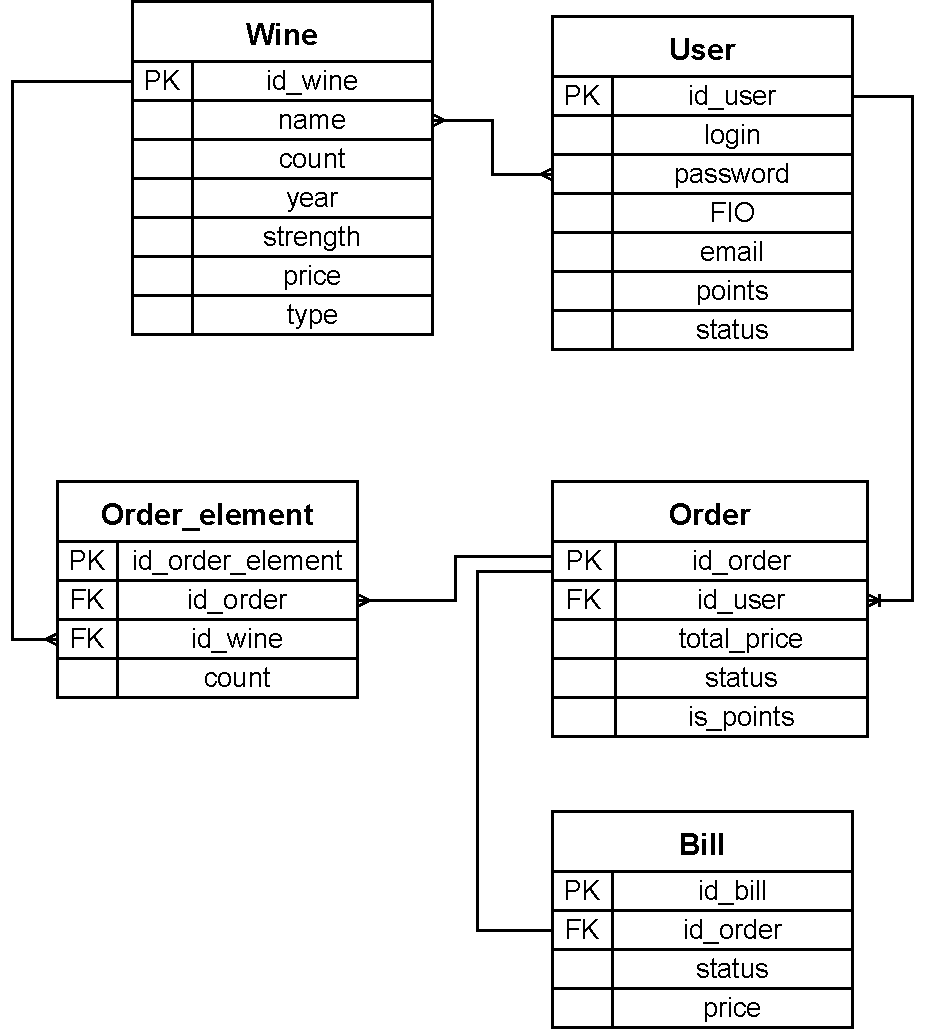
\includegraphics[scale=0.8]{inc/img/er_db.pdf}
	\caption{ER диаграмма базы данных}
	\label{img:er-db}
\end{figure} 

\subsection{Описание проектируемых ограничений целостности базы данных}
\begin{enumerate}[label=\arabic*)]
	\item Таблица вин wine.

     Данные поля не могут быть пустыми:
     \begin{itemize}
         \item[--] id\_wine -- номер вина, первичный ключ;
         \item[--] name -- название вина, символьный тип;
         \item[--] year -- год создания вина, целочисленный тип;
         \item[--] price -- цена вина, целочисленный тип;
         \item[--] country -- страна вина, символьный тип;
         \item[--] type -- сорт вина, символьный тип.
     \end{itemize}

     Поле count по умолчанию равно 10.
 
	\item Таблица пользователей user.

Поля login, password и email должны быть не пустыми. Поле email должно быть заполнено по шаблону электронной почты вида "*@*.*"{}. Где значок * означает любое количество символов. Количество баллов в таблице по умолчанию 0, а статус у пользователя по умолчанию стоит customer.

	\item Таблица заказов order.

Статус заказа не может быть пустым.

        
        \item Таблица счетов bill.
        
        Статус счета не может быть пустым.

\end{enumerate}
\section{Требование к программе}

Для успешной реализации поставленной задачи программа должна
предоставлять следующие возможности для незарегистрированного пользователя:
\begin{itemize}
    \item[--] авторизация;
    \item[--] регистрация;
    \item[--] вывод списка всех вин.
\end{itemize}

У незарегистрированного пользователя есть доступ к просмотру таблицы Wine. А также на добавление в таблицу User.

Зарегистрированный пользователь должен иметь следующие возможности:
\begin{itemize}
    \item[--] авторизация;
    \item[--] вывод списка всех вин;
    \item[--] добавление вина в заказ;
    \item[--] удаление вина из заказа;
    \item[--] просмотр заказа;
    \item[--] оформление заказа.
\end{itemize}

У зарегистрированного пользователя есть доступ к просмотру таблицы Wine, на добавление в таблицу User, есть доступ на создание, удаление и просмотр любимых вин, есть доступ на просмотр и добавление/удаление полей к таблицам Order и Order\_element, а также на вставку и просмотр счета.

Возможности администратора:
\begin{itemize}
    \item[--] авторизация;
    \item[--] добавление вина в каталог; 
    \item[--] удаление вина из каталога; 
    \item[--] обновление вина в каталоге;
    \item[--] подтверждение оплаты счета;
    \item[--] обновление бонусов у пользователя.
\end{itemize}

У администратора есть все права доступа над всеми таблицами базы данных.

\section{Проектирование приложения}

Программу можно разделить на 2 основные части:
\begin{itemize}
    \item[--] front-end – приложение с которым взаимодействует пользователь,
отображение данных;
\item[--] back-end – взаимодействие с базой данных: получение, удаление и
изменение данных.
\end{itemize}

На рисунке \ref{img:uml} представлена UML диаграмма классов моделей
и представлений.
\begin{figure}[H]
	\centering
	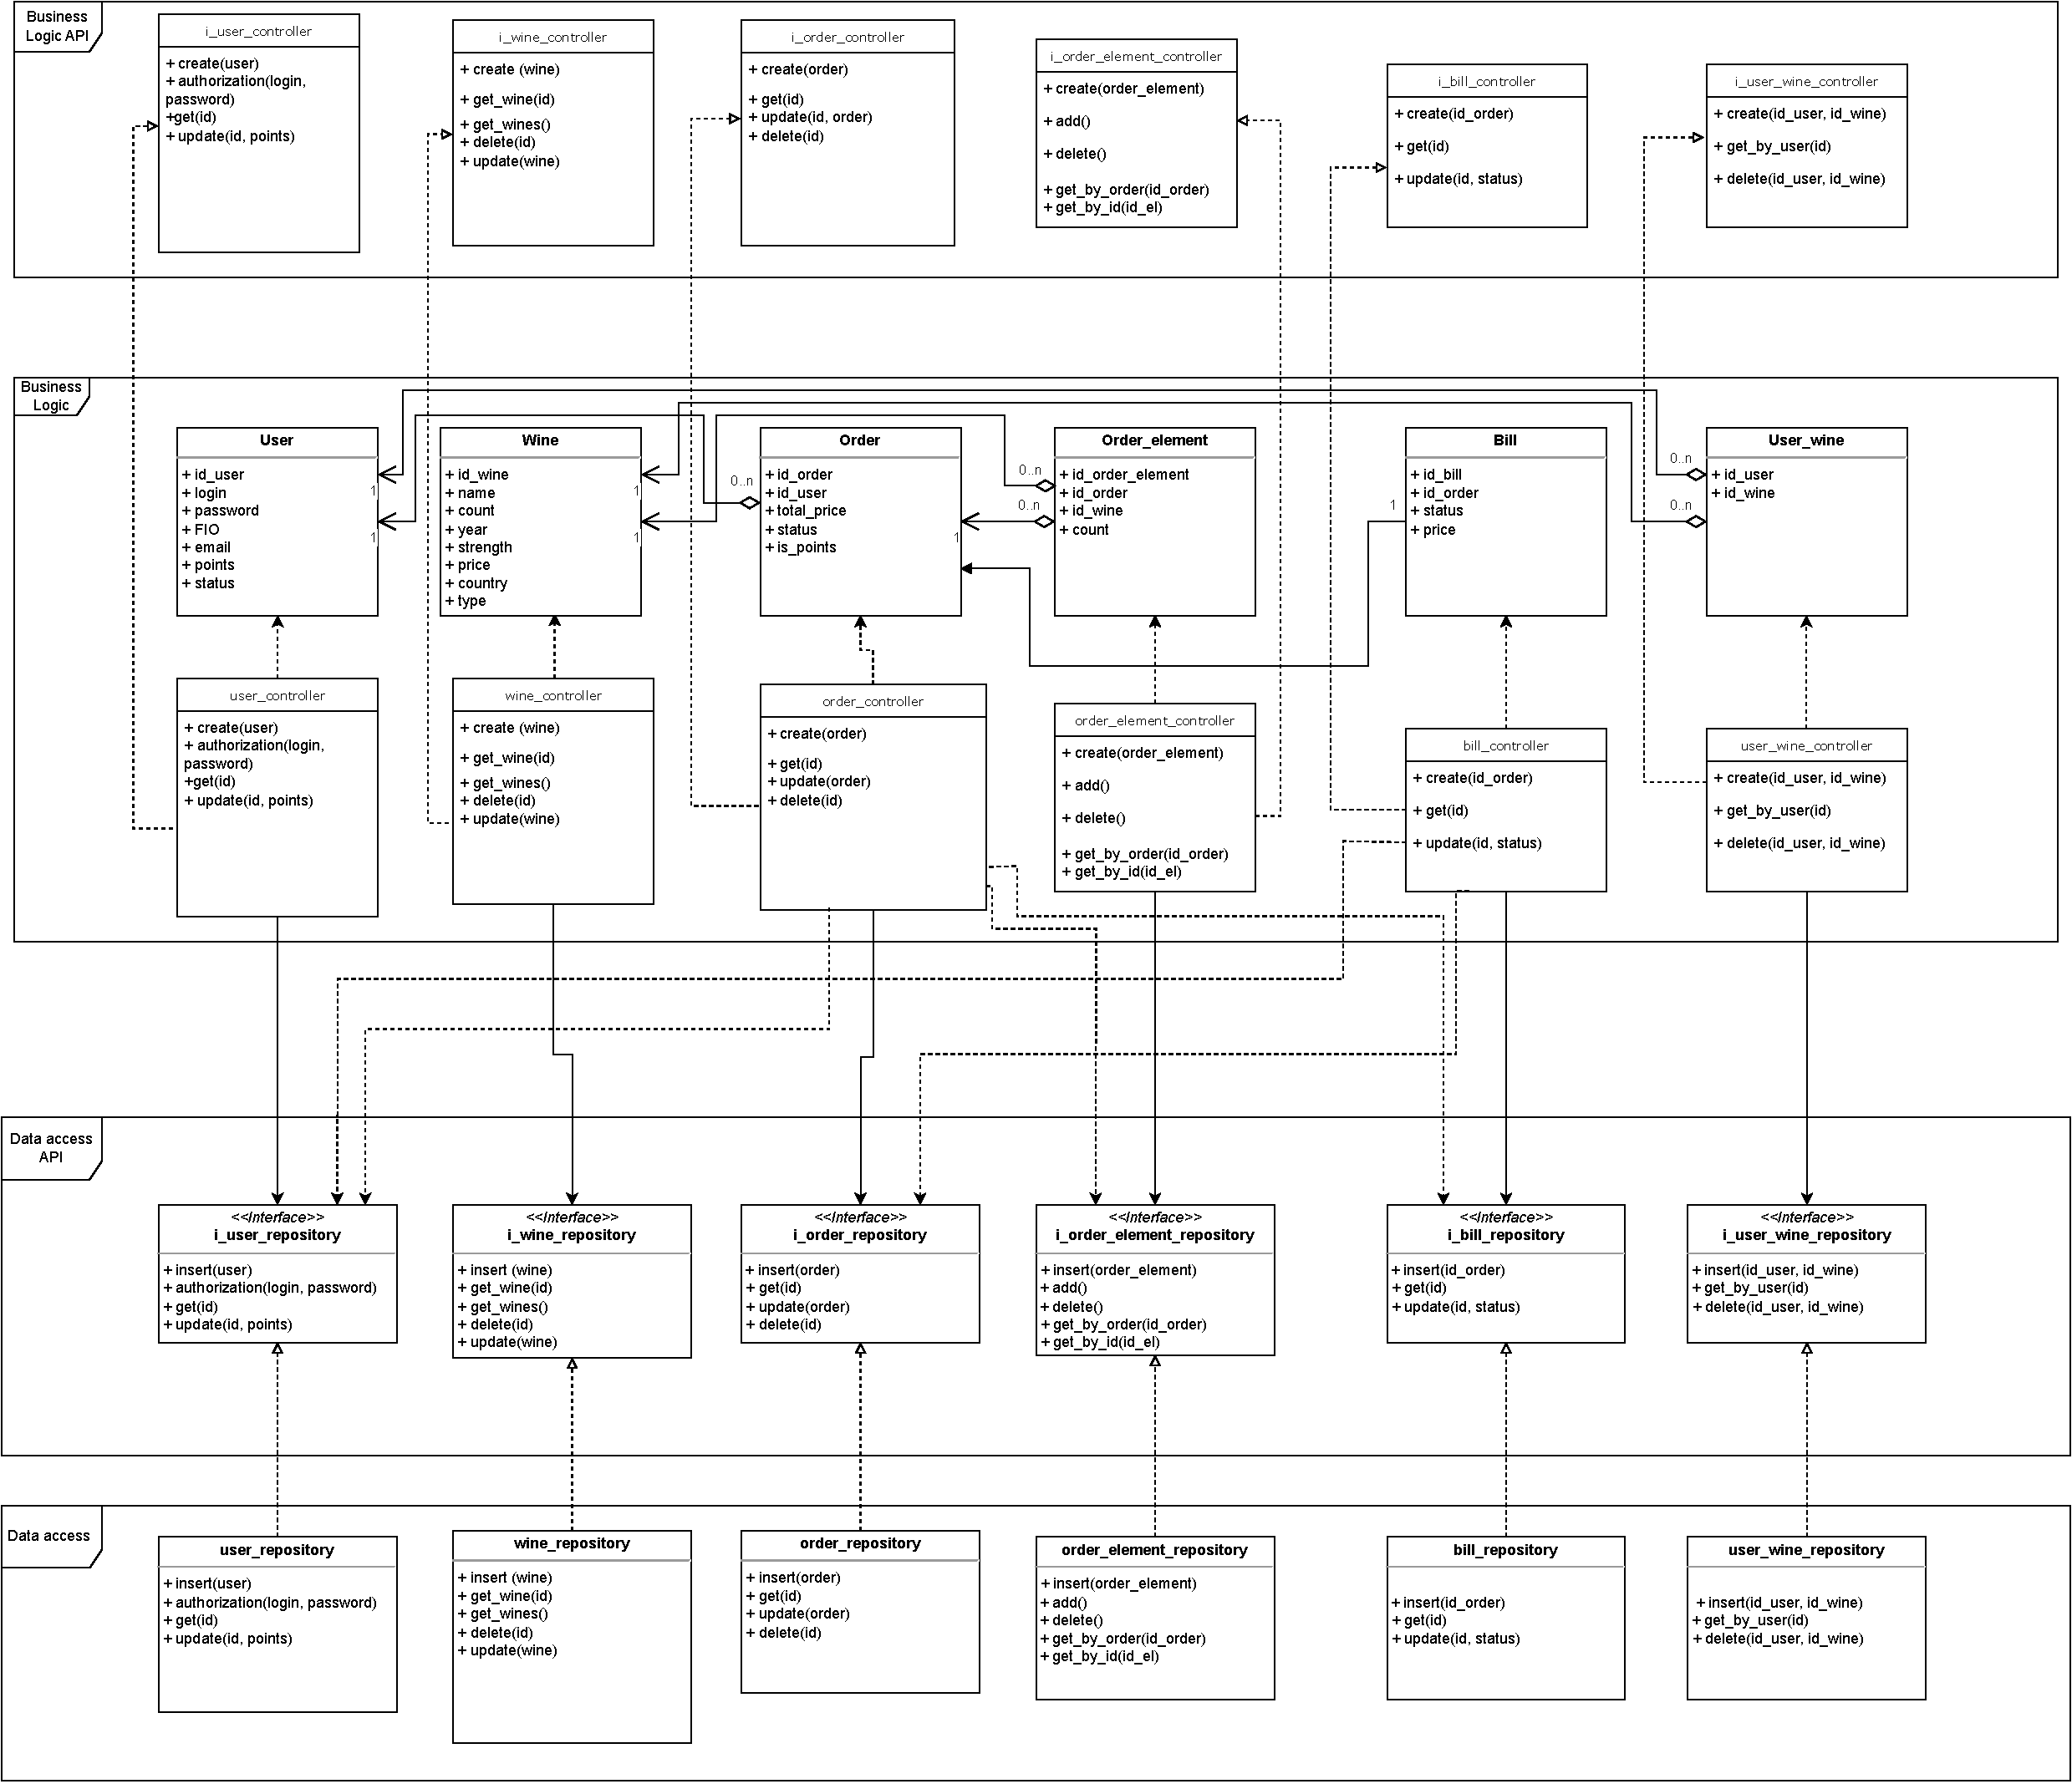
\includegraphics[scale=0.40]{inc/img/uml.pdf}
	\caption{UML диаграмма}
	\label{img:uml}
\end{figure} 

\section{Разработка триггера базы данных}

Был спроектирован триггер для создания нового элемента в заказе. При создании элемента заказа, надо следить, чтобы данное вино не находилось уже в данном заказе, чтобы не было ситуаций, когда в заказе несколько элементов с одинаковыми винами, но разным количеством товара. Если покупатель хочет изменить количество товара в элементе заказа, то ему предоставляются функции по увелечению и уменьшению количества элементов заказа. Также необходимо следить, чтобы покупатель не положил в заказ вина больше, чем есть на складе. Чтобы обеспечить данные проверки был спроектирован триггер, который срабатывает при создании нового элемента заказа. Схема данного триггера представлена на рисунке \ref{img:tr}.

\begin{figure}[H]
	\centering
	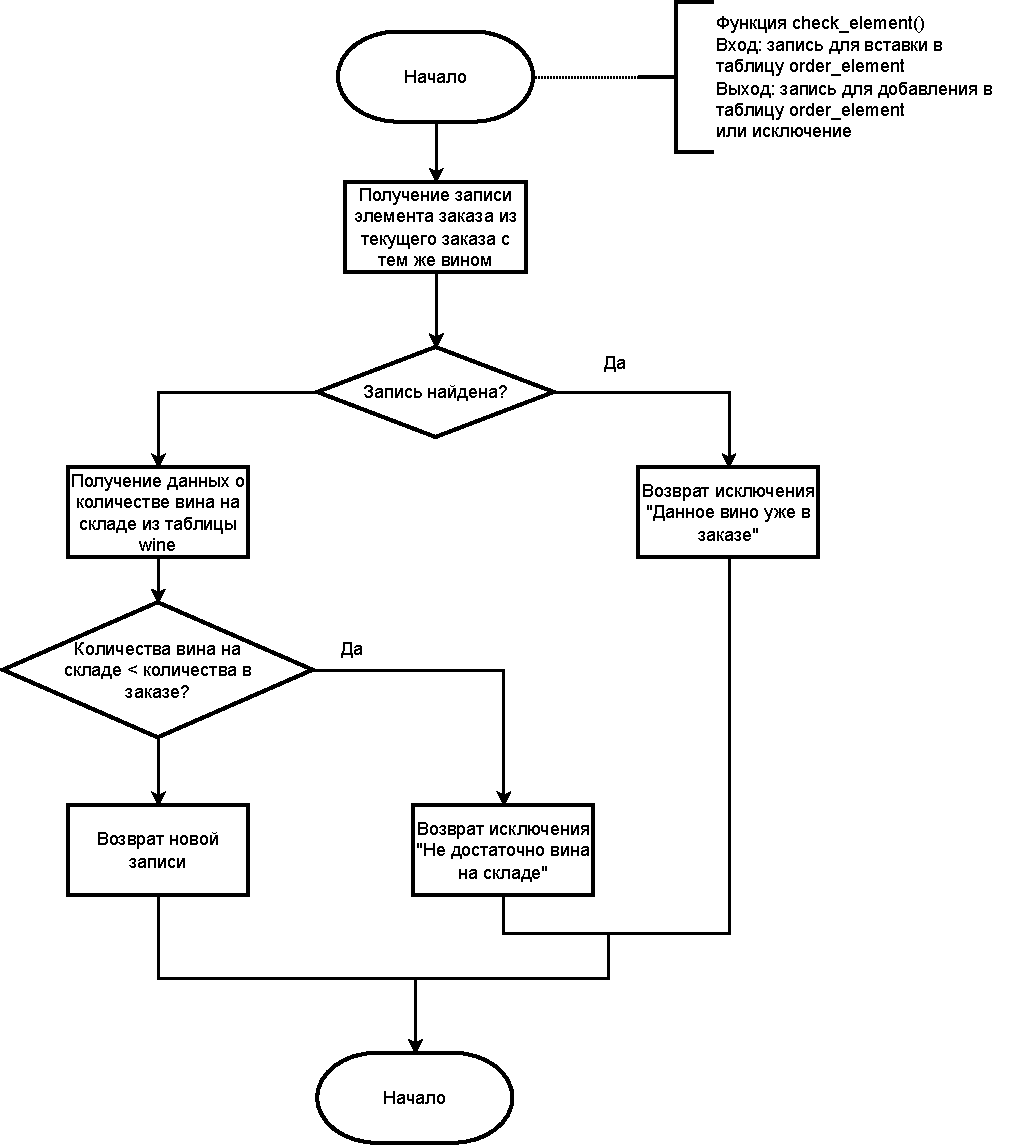
\includegraphics[scale=1]{inc/img/tr.pdf}
	\caption{Схема алгоритма функции спроектированного триггера, срабатывающего при добавлении элемента заказа}
	\label{img:tr}
\end{figure} 
